\documentclass[11pt,paper=a4,final]{scrartcl}
\usepackage[utf8]{inputenc}
\usepackage{geometry}           %allows us to specify the 'seitenrand'
\usepackage{graphicx}           %package used to include graphics
\usepackage{hyperref}           %used to make klickable links
\usepackage{listings}
\usepackage{tabularx}
\usepackage{pdflscape}
\usepackage[figuresright]{rotating}
\usepackage{nameref}
\usepackage{longtable}
\usepackage{enumitem}
\usepackage{footnote}
% Make the document German
\usepackage{ngerman}
% allow rowspan
\usepackage{multirow}

\hypersetup{
    colorlinks,
    citecolor=black,
    filecolor=black,
    linkcolor=black,
    urlcolor=black
}

\usepackage{fancyhdr}
\pagestyle{fancy}
% \setlength{\parskip}{0pt}
% \setlength{\baselineskip}{0pt}
%\parindent 0pt 
%\parskip 11pt
%\parsep 0pt 
%\itemsep 0pt 
%\topsep 0pt 

\geometry{a4paper, top=20mm, right=20mm, bottom=20mm, left=20mm}

%defining header and footer
\fancyhf{}      %delete default values
\setlength{\headwidth}{\textwidth}      %header and footer width equal the text width
%\fancyhead[LE,LO]{\includegraphics[scale=0.6]{header.png}}
\fancyhead[LE,LO]{Roland Peka Rytz, Niklaus Manuel Hofer}
\fancyhead[RE,RO]{Chromatographie}
\fancyfoot[CE,CO]{Speicherdatum: \today{}}
\fancyfoot[RE,RO]{\thepage}

%New page for every section
%\let\stdsection\section
%\renewcommand\section{\newpage\stdsection}

\title{Chromatographie}
\author{Roland Peka Rytz, Niklaus Manuel Hofer}
\date{\today{}}

\begin{document}
\maketitle

\section{Messwerte, Beobachtungen}
\subsection{Messwerte}
Genauigkeit der Chromatographie-Platten: unbekannt\\
Genauigkeit der Messung (siehe unten): \( \pm 0.3cm\) \\
Ungenauigkeit beim Vermessen der L\"osungsmittel-Front: vernachl\"assigbar \\
Die Temepratur im Arbeitszimmer betrug: \(20^\circ C \pm 3^\circ C\)
\subsection{Stifte und gegebene Mischung}
\begin{savenotes} %Handles footnotes within tables
  \begin{table}[ht!]
    \centering
    \begin{tabular}{|l|l|l|l|}
      \hline
    \bf Farbe Nr.	& \bf Teilfarbe	& \bf \(R_{Lsm}\)		& \bf Distanz (\(R_x\))	\\ \hline
      1 (hellblau)	& hellblau	& \multirow{6}{*}{6.1 cm }	& 4.0 cm \(\pm 3 mm \)	\\ \cline{1-2} \cline{4-4}
      2 (dunkelgr\"un)	& dunkelgr\"un	&				& 5.8 cm \(\pm 3 mm \)	\\ \cline{1-2} \cline{4-4}
      \multirow{2}{*}{3 (rot) }
			& pink		&				& 4.6 cm \(\pm 3 mm \)	\\ 
			& orange	&				& 6.1 cm 		\\ \cline{1-2} \cline{4-4}
      \multirow{2}{*}{4 (hellgr\"un) }
 			& hellblau	&				& 3.3 cm \(\pm 3 mm \)	\\
			& gelb		&				& 6.1 cm		\\ \hline
      5 (gelb)		& orange	& \multirow{10}{*}{6.1 cm }	& 6.1 cm		\\ \cline{1-2} \cline{4-4}
      \multirow{4}{*}{6 (braun)}
			& Violett	&				& 0.7 cm \(\pm 3 mm \)	\\
			& hellblau	&				& 2.7 cm \(\pm 3 mm \)	\\
      			& pink		&				& 3.9 cm \(\pm 3 mm \)	\\
      			& Orange	&				& 6.1 cm 		\\ \cline{1-2} \cline{4-4}
      \multirow{2}{*}{7 (schwarz}
      			& gelb		&				& 4.0 cm \(\pm 6 mm \)	\\
      			& schwarz	&				& 6.1 cm		\\ \cline{1-2} \cline{4-4}
      \multirow{3}{*}{8 (rot)}
      			& dunkelpink	& 				& 1.6 cm \(\pm 3 mm \)	\\ 
      			& hellpink	&				& 4.7 cm \(\pm 3 mm \)	\\
      			& orange	&				& 6.1 cm		\\ \hline
      9 (t\"urkis)	& t\"urkis	& \multirow{6}{*}{6.0 cm }	& 3.5 cm \(\pm 3 mm \)	\\ \cline{1-2} \cline{4-4}
       10 (orange)	& orange	& 				& 6.0 cm		\\ \cline{1-2} \cline{4-4}
      \multirow{3}{*}{11 (Violett)}
      			& dunkelpink	&				& 1.9 cm \(\pm 3 mm \)	\\
      			& hellpink	&				& 2.3 cm \(\pm 3 mm \)	\\
      			& blau		&				& 6.0 cm		\\ \cline{1-2} \cline{4-4}
      12 (pink)		& pink		&				& 0.3 cm \(\pm 1 mm \)	\\ \hline
      \multirow{4}{*}{Mischung 4}
      			& Violett	& \multirow{4}{*}{6.0 cm }	& 0.6 cm \(\pm 2 mm \)	\\
      			& dunkelpink	&				& 1.2 cm \(\pm 3 mm \)	\\
			& blau		& 				& 2.7 cm \(\pm 3 mm \)	\\
      			& hellpink	& 				& 3.6 cm \(\pm 3 mm \)	\\ \hline
      	
    \end{tabular}
    \caption{Messergebnisse}
    \end{table}
\end{savenotes}

\subsection{Eigene Mischungen}
\begin{savenotes}
  \begin{table}[ht!]
    \centering
    \begin{tabular}{|l|l|}
      \hline
      \bf Name & \bf Verwendete Stifte	\\ \hline
      A & 5 + 6 			\\ \hline
      B & 10 + 5			\\ \hline
      C & 10 + 6 			\\ \hline
      D & 6 + 5 + 10			\\ \hline
      E & 6 + 3				\\ \hline
      F & (unbekannt)			\\ \hline
      G & 6 + 11			\\ \hline
      H & 6 + 8				\\ \hline
    \end{tabular}
    \caption{Eigene Mischungen}
  \end{table}
\end{savenotes}

\begin{savenotes}
  \begin{table}[ht!]
    \centering
    \begin{tabular}{|l|l|l|l|}
      \hline
      \bf Mischung	& \bf Teilfarbe	& \bf \(R_{Lsm}\)		& \bf Distanz (\(R_x\))	\\ \hline
      \multirow{4}{*}{A}
			& Violett	& \multirow{13}{*}{4.8 cm }	& 0.9 cm \(\pm 3 mm \)	\\
      			& blau		& 				& 2.6 cm \(\pm 3 mm \)	\\
      			& pink		&				& 3.1 cm \(\pm 3 mm \)	\\
      			& orange	&				& 4.8 cm 		\\ \cline{1-2} \cline{4-4}
       B		& orange	&				& 4.8 cm		\\ \cline{1-2} \cline{4-4}
      \multirow{4}{*}{C}
			& Violett	& 				& 0.9 cm \(\pm 3 mm \)	\\
      			& blau		& 				& 2.6 cm \(\pm 3 mm \)	\\
      			& pink		&				& 3.1 cm \(\pm 3 mm \)	\\
      			& orange	&				& 4.8 cm 		\\ \cline{1-2} \cline{4-4}
      \multirow{4}{*}{D}
			& Violett	&				& 0.9 cm \(\pm 3 mm \)	\\
      			& blau		& 				& 2.6 cm \(\pm 3 mm \)	\\
      			& pink		&				& 3.1 cm \(\pm 3 mm \)	\\
      			& orange	&				& 4.8 cm 		\\ \hline
      \multirow{4}{*}{E}
			& Violett	& \multirow{18}{*}{4.6 cm }	& 1.2 cm \(\pm 3 mm \)	\\
      			& blau		& 				& 2.7 cm \(\pm 3 mm \)	\\
      			& pink		&				& 3.3 cm \(\pm 3 mm \)	\\
			      & orange	&				& 4.6 cm 		\\ \cline{1-2} \cline{4-4}
      \multirow{4}{*}{F}
			& Violett	&				& 1.2 cm \(\pm 3 mm \)	\\
      			& blau		& 				& 2.7 cm \(\pm 3 mm \)	\\
      			& pink		&				& 3.5 cm \(\pm 3 mm \)	\\
			& orange	&				& 4.6 cm 		\\ \cline{1-2} \cline{4-4}
      \multirow{5}{*}{G}
			& Violett	&				& 1.3 cm \(\pm 3 mm \)	\\
      			& dunkelpink 	&				& 1.7 cm \(\pm 3 mm \)	\\
			& blau		&				& 2.6 cm \(\pm 3 mm \)	\\
      			& hellpink	& 				& 3.1 cm \(\pm 3 mm \)	\\
      			& orange	&				& 4.6 cm		\\ \cline{1-2} \cline{4-4}
      \multirow{5}{*}{F}
			& Violett	&				& 1.2 cm \(\pm 3 mm \)	\\
      			& dunkelpink 	&				& 1.5 cm \(\pm 3 mm \)	\\
      			& blau		& 				& 2.7 cm \(\pm 3 mm \)	\\
      			& pink		&				& 3.5 cm \(\pm 3 mm \)	\\
			& orange	&				& 4.6 cm 		\\ \hline

    \end{tabular}
    \caption{Messergebnisse der Mischungen}
  \end{table}
\end{savenotes}

\section{Berechnungen, Resultate}
Die Formel zur Berechnung von \(R_f\) ist wie folgt: \(R_f = \frac{R_x}{R_{Lsm}} \) \\
Wobei gilt:\\
\(R_x\): Laufstrecke der Substanz\\
\(R_{Lsm}\): Laufstrecke des L\"osungsmittles
\subsection{Stifte und gegebene Mischung}
\begin{savenotes} %Handles footnotes within tables
  \begin{table}[ht!]
    \centering
    \begin{tabular}{|l|l|l|l|l|}
      \hline
    \bf Farbe Nr.	& \bf Teilfarbe	& \bf \(R_{Lsm}\)		& \bf Distanz (\(R_x\))	& \bf \(R_f\)		\\ \hline
      1 (hellblau)	& hellblau	& \multirow{6}{*}{6.1 cm }	& 4.0 cm \(\pm 3 mm \)	& 0.607 - 0.705		\\ \cline{1-2} \cline{4-5}
      2 (dunkelgr\"un)	& dunkelgr\"un	&				& 5.8 cm \(\pm 3 mm \)	& 0.902 - 1.000		\\ \cline{1-2} \cline{4-5}
      \multirow{2}{*}{3 (rot) }
			& pink		&				& 4.6 cm \(\pm 3 mm \)	& 0.705 - 0.803		\\ 
			& orange	&				& 6.1 cm 		& 1.00 (nicht definiert)\\ \cline{1-2} \cline{4-5}
      \multirow{2}{*}{4 (hellgr\"un) }
 			& hellblau	&				& 3.3 cm \(\pm 3 mm \)	& 0.500 - 0.600		\\
			& gelb		&				& 6.1 cm		& 1.00 (nicht definiert)\\ \hline
      5 (gelb)		& orange	& \multirow{10}{*}{6.1 cm }	& 6.1 cm		& 1.00 (nicht definiert)\\ \cline{1-2} \cline{4-5}
      \multirow{4}{*}{6 (braun)}
			& Violett	&				& 0.7 cm \(\pm 3 mm \)	& 0.066 - 0.164		\\
			& hellblau	&				& 2.7 cm \(\pm 3 mm \)	& 0.393 - 0.492		\\
      			& pink		&				& 3.9 cm \(\pm 3 mm \)	& 0.590 - 0.689		\\
      			& Orange	&				& 6.1 cm 		& 1.00 (nicht definiert)\\ \cline{1-2} \cline{4-5}
      \multirow{2}{*}{7 (schwarz}
      			& gelb		&				& 4.0 cm \(\pm 6 mm \)	& 0.557 - 0.754		\\
      			& schwarz	&				& 6.1 cm		& 1.00 (nicht definiert)\\ \cline{1-2} \cline{4-5}
      \multirow{3}{*}{8 (rot)}
      			& dunkelpink	& 				& 1.6 cm \(\pm 3 mm \)	& 0.213 - 0.311		\\ 
      			& hellpink	&				& 4.7 cm \(\pm 3 mm \)	& 0.721 - 0.820		\\
      			& orange	&				& 6.1 cm		& 1.00 (nicht definiert)\\ \hline
      9 (t\"urkis)	& t\"urkis	& \multirow{6}{*}{6.0 cm }	& 3.5 cm \(\pm 3 mm \)	& 0.533 - 0.633		\\ \cline{1-2} \cline{4-5}
       10 (orange)	& orange	& 				& 6.0 cm		& 1.00 (nicht definiert)\\ \cline{1-2} \cline{4-5}
      \multirow{3}{*}{11 (Violett)}
      			& dunkelpink	&				& 1.9 cm \(\pm 3 mm \)	& 0.266 - 0.366		\\
      			& hellpink	&				& 2.3 cm \(\pm 3 mm \)	& 0.333 - 0.433		\\
      			& blau		&				& 6.0 cm		& 1.00 (nicht definiert \\ \cline{1-2} \cline{4-5}
      12 (pink)		& pink		&				& 0.3 cm \(\pm 1 mm \)	& 0.033 - 0.066		\\ \hline
      \multirow{4}{*}{Mischung 4}
      			& Violett	& \multirow{4}{*}{6.0 cm }	& 0.6 cm \(\pm 2 mm \)	& 0.066 - 0.133		\\
      			& dunkelpink	&				& 1.2 cm \(\pm 3 mm \)	& 0.150 - 0.250		\\
			& blau		& 				& 2.7 cm \(\pm 3 mm \)	& 0.400 - 0.500		\\
      			& hellpink	& 				& 3.6 cm \(\pm 3 mm \)	& 0.550 - 0.650		\\ \hline
      	
    \end{tabular}
    \caption{Berechnung der Rf-Werte}
    \end{table}
\end{savenotes}
\subsection{Eigene Mischungen}
\begin{savenotes}
  \begin{table}[ht!]
    \centering
    \begin{tabular}{|l|l|l|l|l|}
      \hline
      \bf Mischung	& \bf Teilfarbe	& \bf \(R_{Lsm}\)		& \bf Distanz (\(R_x\))	& \(R_f\)		\\ \hline
      \multirow{4}{*}{A}
			& Violett	& \multirow{13}{*}{4.8 cm }	& 0.9 cm \(\pm 3 mm \)	& 0.125 - 0.250		\\
      			& blau		& 				& 2.6 cm \(\pm 3 mm \)	& 0.479 - 0.604		\\
      			& pink		&				& 3.1 cm \(\pm 3 mm \)	& 0.583 - 0.708		\\
      			& orange	&				& 4.8 cm 		& 1.00 (nicht definiert)\\ \cline{1-2} \cline{4-5}
       B		& orange	&				& 4.8 cm		& 1.00 (nicht definiert)\\ \cline{1-2} \cline{4-5}
      \multirow{4}{*}{C}
			& Violett	& 				& 0.9 cm \(\pm 3 mm \)	& 0.125 - 0.250		\\
      			& blau		& 				& 2.6 cm \(\pm 3 mm \)	& 0.479 - 0.604		\\
      			& pink		&				& 3.1 cm \(\pm 3 mm \)	& 0.583 - 0.708		\\
      			& orange	&				& 4.8 cm 		& 1.00 (nicht definiert)\\ \cline{1-2} \cline{4-5}
      \multirow{4}{*}{D}
			& Violett	&				& 0.9 cm \(\pm 3 mm \)	& 0.125 - 0.250		\\
      			& blau		& 				& 2.6 cm \(\pm 3 mm \)	& 0.479 - 0.604		\\
      			& pink		&				& 3.1 cm \(\pm 3 mm \)	& 0.583 - 0.708		\\
      			& orange	&				& 4.8 cm 		& 1.00 (nicht definiert)\\ \hline
      \multirow{4}{*}{E}
			& Violett	& \multirow{18}{*}{4.6 cm }	& 1.2 cm \(\pm 3 mm \)	& 0.196 - 0.326		\\
      			& blau		& 				& 2.7 cm \(\pm 3 mm \)	& 0.522 - 0.652		\\
      			& pink		&				& 3.3 cm \(\pm 3 mm \)	& 0.652 - 0.782		\\
			      & orange	&				& 4.6 cm 		& 1.00 (nicht definiert)\\ \cline{1-2} \cline{4-5}
      \multirow{4}{*}{F}
			& Violett	&				& 1.2 cm \(\pm 3 mm \)	& 0.196 - 0.326		\\
      			& blau		& 				& 2.7 cm \(\pm 3 mm \)	& 0.522 - 0.652		\\
      			& pink		&				& 3.5 cm \(\pm 3 mm \)	& 0.696 - 0.826		\\
			& orange	&				& 4.6 cm 		& 1.00 (nicht definiert)\\ \cline{1-2} \cline{4-5}
      \multirow{5}{*}{G}
			& Violett	&				& 1.3 cm \(\pm 3 mm \)	& 0.217 - 0.348		\\
      			& dunkelpink 	&				& 1.7 cm \(\pm 3 mm \)	& 0.304 - 0.435		\\
			& blau		&				& 2.6 cm \(\pm 3 mm \)	& 0.500 - 0.630		\\
      			& hellpink	& 				& 3.1 cm \(\pm 3 mm \)	& 0.609 - 0.739		\\
      			& orange	&				& 4.6 cm		& 1.00 (nicht definiert \\ \cline{1-2} \cline{4-5}
      \multirow{5}{*}{F}
			& Violett	&				& 1.2 cm \(\pm 3 mm \)	& 0.196 - 0.326		\\
      			& dunkelpink 	&				& 1.5 cm \(\pm 3 mm \)	& 0.261 - 0.391		\\
      			& blau		& 				& 2.7 cm \(\pm 3 mm \)	& 0.522 - 0.652		\\
      			& pink		&				& 3.5 cm \(\pm 3 mm \)	& 0.696 - 0.826		\\
			& orange	&				& 4.6 cm 		& 1.00 (nicht definiert)\\ \hline

    \end{tabular}
    \caption{Messergebnisse der Mischungen}
  \end{table}
\end{savenotes}

\section{Fehlerabsch\"atzung}
\begin{itemize}
  \item Die Genauigkeit der Chromatographie-Platten ist leider unbekannt.
  \item Die Messung der \( R_X \) Werte ist aber ohnehin nicht besonders genau. Auch, da nicht genau klar ist wo diese gemessen werden. Einige Farbklekse laufen nach oben langsam aus.
\end{itemize}

\section{anhang}
\begin{figure}[h!]
  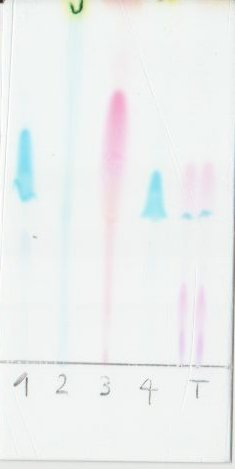
\includegraphics{1-4}
  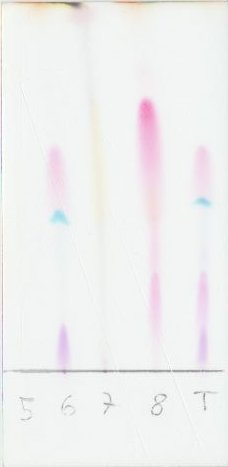
\includegraphics{5-8}
  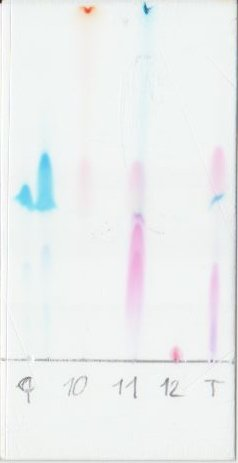
\includegraphics{9-12}
  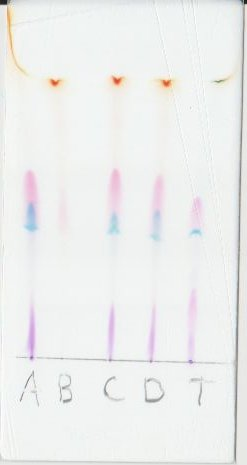
\includegraphics{a-d}
  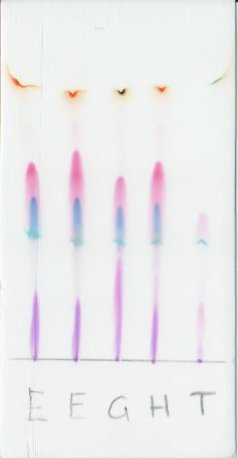
\includegraphics{e-h}
  \caption{Stifte 1 bis 4}
  \caption{Stifte 5 bis 8}
  \caption{Stifte 9 bis 12}
  \caption{Mischungen A bis D}
  \caption{Mischungen E bis H}
\end{figure}
\end{document}
